\documentclass[12pt,a4paper, twocolumn]{article}



\usepackage{graphicx}
\usepackage[english]{babel}
\usepackage{datetime}
\usepackage{geometry}
\usepackage{setspace}
\usepackage[hidelinks]{hyperref}

\geometry{
	a4paper,
	total={170mm,257mm},
	left=30mm,
	right=30mm,
	top=20mm,
}

\graphicspath{ {./images/} }

\newdateformat{monthyeardate}{%
	\monthname[\THEMONTH], \THEYEAR}

\onehalfspacing

\begin{document}
\begin{titlepage}
	\centering
	 \textsc{\'Ecole polytechnique f\'ed\'erale de Lausanne}\\
	 \textsc{Center for Digital Education}\\
	\vspace{2.5cm}
	
\includegraphics[scale=0.3]{Logo}\par
	\vspace{20pt}
	\hrule
	\vspace{5pt}
	{\LARGE\bfseries Analysing the FIFA World Cup 2018\par}
	\vspace{5pt}
	\hrule
	\vspace{10pt}
	
	\large \textbf{Network Tour of Data Science}\\
	\monthyeardate \today\par

	\vfill
	{\Large \textbf{Team 09}\par}

	\vspace{2cm}

% Bottom of the page
	Supervisors:\par
	\textbf{XXX} \\
	\textbf{XXX} 
\end{titlepage}

\section{Introduction}

\section{Data Analysis}

\section{Task xy}

\section{Identifying players in each team}
When analysing a world cup only based on the links and number of views from Wikipedia one interesting questions we asked ourself is, if it is possible to identify the players of each team just by using this specific network structure. 

In this section we will show two approaches that lead in different ways to the objective of the above-mentioned thesis. 

\subsection{Heat Signal}
In our first approach to identify the players of each team we were using a heat filter. For this method we are using the network of hyperlinks where each player is connected to the page of his team. The aim of this method is to apply a delta impulse as a heat signal on a certain node, which then will be transmitted to the neighbouring nodes. These neighbouring nodes ideally have a close relationship to the initial note, in our case the same national team. 
\par
After applying the heat signal on the network we had a continues signal on our network. Because each team is only allowed to have a maximum number of 23 players, we set an upper limit for the heat, in order to filter the 23 most heat transmitted nodes. Those nodes were when our prediction for the different players in the same team. 
\par
It turned out that this method worked very good and when comparing the results with the actual true labels, we obtained an accuracy of mostly over 95 percent. In figure \ref{fig:cluster_4} we can see the predicted nodes for the Croatian national team in the network. The yellow nodes are nodes that were predicted right, where the green nodes represent nodes that were not assigned even though they belong to the team.  

\begin{figure}[h!]
	\centering
	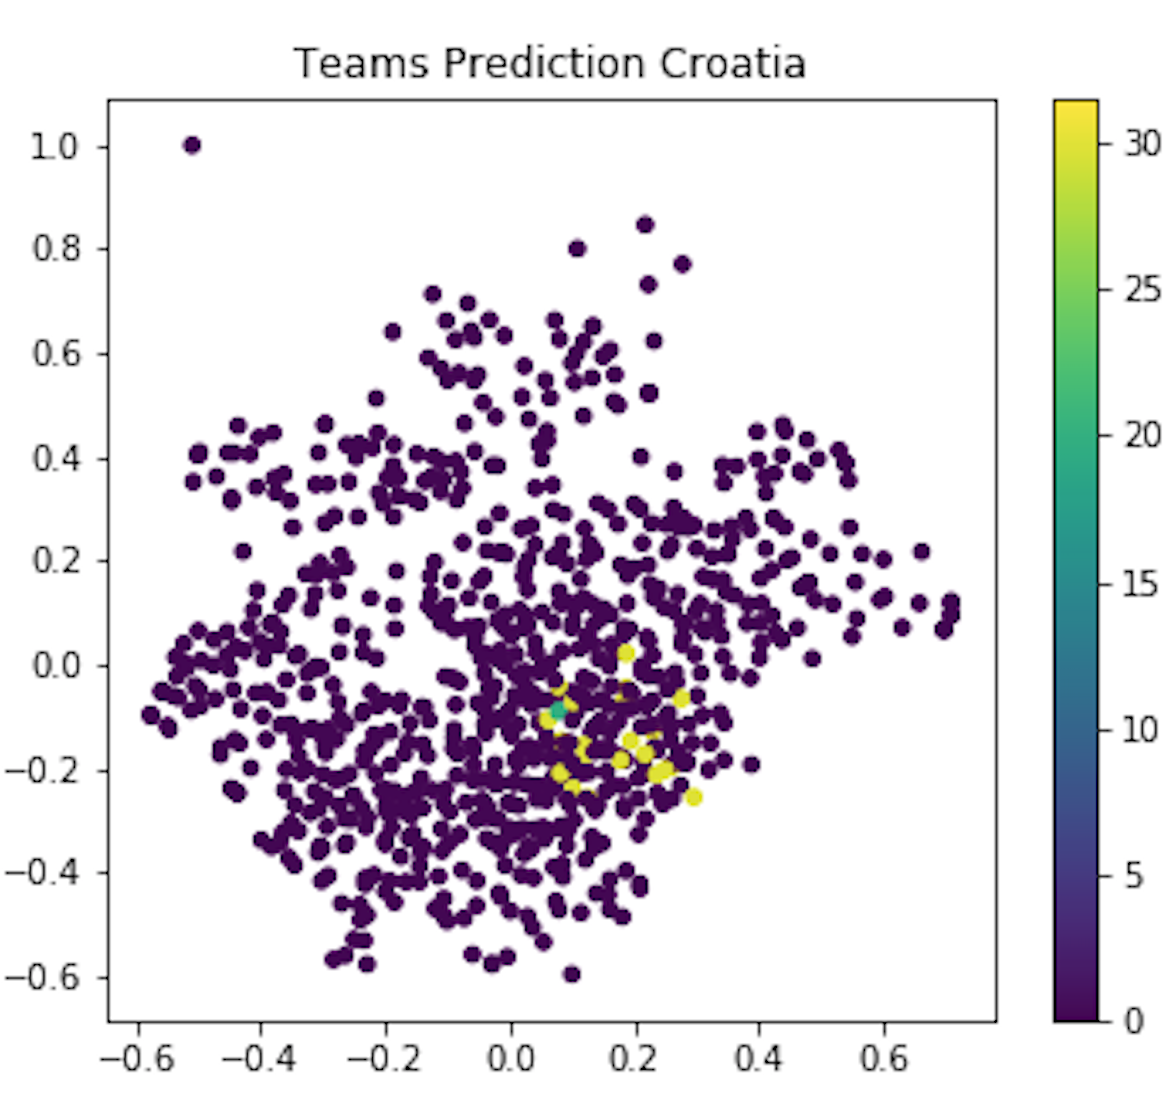
\includegraphics[width=0.5\textwidth]{ClusterCroatia.png}
	\caption{Prediction of Croatian national team in hole network}
	\label{fig:cluster_4}
\end{figure}

\subsection{Pearson Correlation}
In our second approach to solve this problem we were using the pearson correlation between the feature vector of each player. Our presumption was that high correlation is mostly due to similar behaviour exhibited by the team structure. In order to visualise the graph in gephi, we reduced the number of edges to only keep the most correlated ones (removed 97\%). The result of the clustering based on the correlation can be seen in figure \ref{fig:cluster_gephi}. 

\begin{figure}[h!]
	\centering
	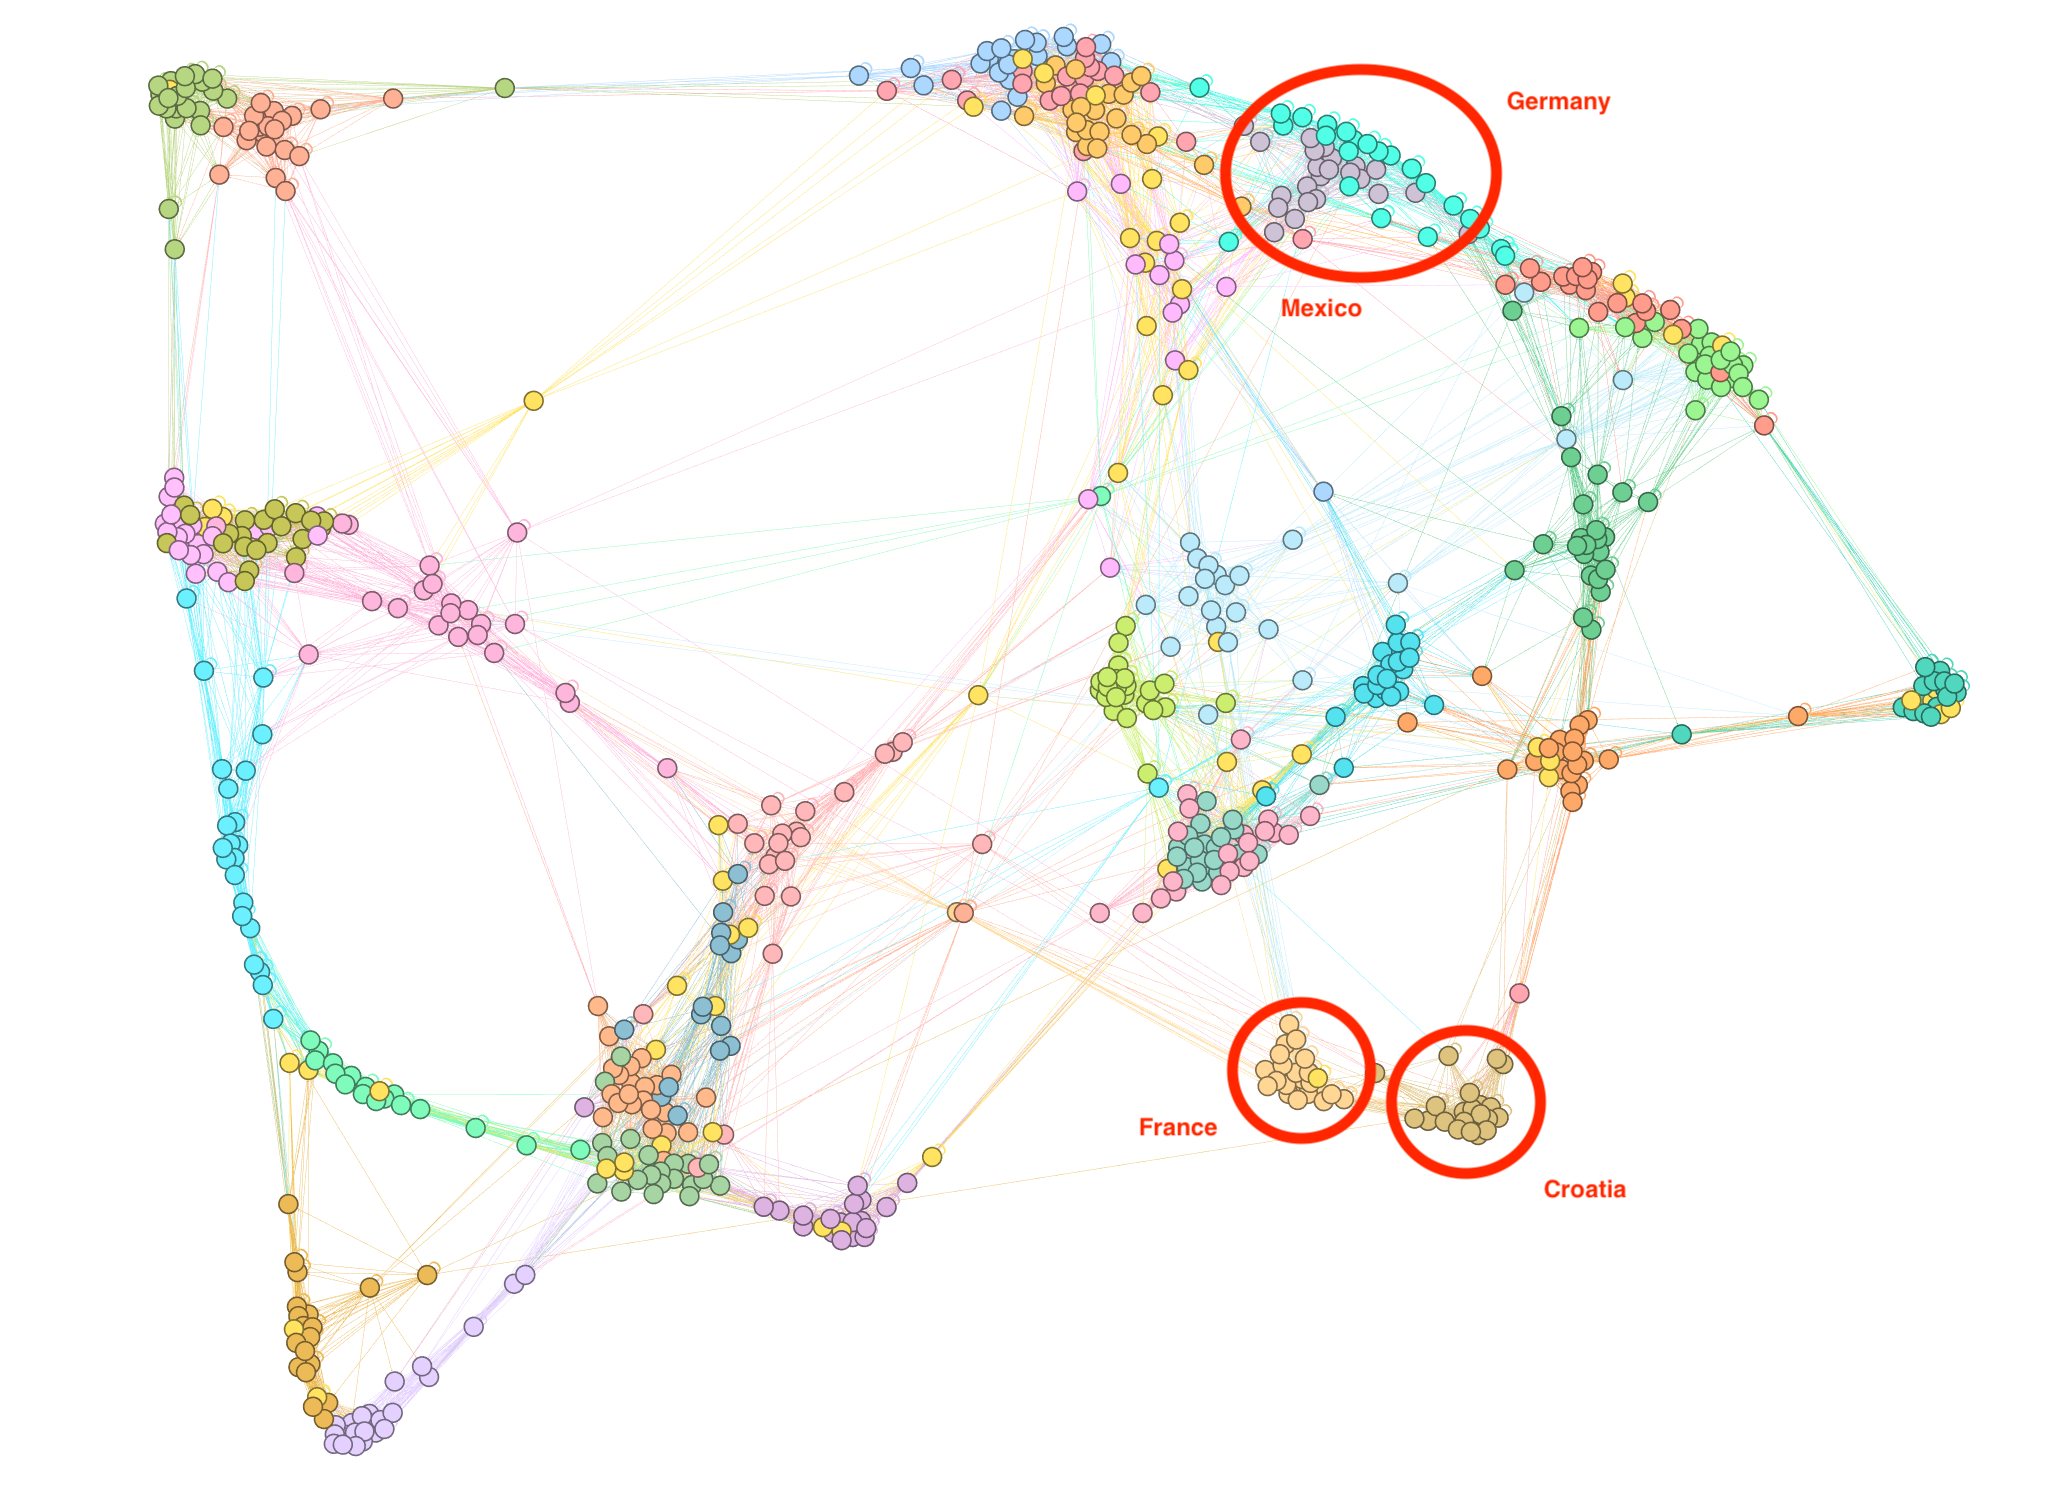
\includegraphics[width=0.5\textwidth]{ClusterGephi.png}
	\caption{Cluster}
	\label{fig:cluster_gephi}
\end{figure}

At a first glance we can observe that the clustering worked for some cluster better than for others. France and Croatia for example were clustered very well while Germany and Mexico are almost one cluster. This is due to the fact some national teams had more matches than others and therefore more unique matches. Mexico and Germany were eliminated after 3/4 matches while Croatia and France had 7 matches. In addition all group matches of the same team were on the same date. Therefore we can hardly distinguish between two teams that had roughly the same amount of matches. 
\par 
As a result both the heat signal and the pearson correlation are ways to identify players of each team. However, the first method achieves slightly better results because it is less linked to the data than the second. 




\section{Data}






\section{Conclusion}



\bibliographystyle{plain}
\bibliography{lit}


\end{document}